\documentclass[conference]{IEEEtran}
\IEEEoverridecommandlockouts

\usepackage{cite}
\usepackage{amsmath,amssymb,amsfonts}
\usepackage{graphicx}
\usepackage{textcomp}
\usepackage{xcolor}
\usepackage{url}

\begin{document}

\title{A Robust Cross-Region Modelling and Validation Framework for Generalisable Cardiovascular Risk Prediction in Type 2 Diabetes}

\author{
\IEEEauthorblockN{Yanbei Zhang}
\IEEEauthorblockA{
SEMTM0045 – Data Science Methods and Practice\\
University of Bristol}
}

\maketitle

\begin{abstract}
Cardiovascular disease is the leading cause of death worldwide. Compared with the general population, patients with type 2 diabetes (T2D) have a higher risk of myocardial infarction, stroke and cardiovascular death. Therefore, risk prediction tools are of great significance for guiding the preventive medication, treatment intensity and follow-up management of this high-risk population. However, the current research on cardiovascular risk prediction for T2D population has not solved the problem of cross-regional application well. Although there are many ready-made models, a key problem remains unresolved: when a trained model is migrated to a new area, it still needs to rely on local data and repeated calibration to achieve satisfactory performance. These models therefore tend to show limited or unstable migrability. For this reason, we propose a multi-area refitting strategy based on the SCORE2-Diabetes framework. The strategy uses unified development data from multiple regions such as Europe, America and Asia. It also adopts internal-external cross-verification (IECV) in model training and fitting, so that the model can be tested across regions at the development stage. Our goal is to evaluate whether this strategy can improve the cross-regional calibration and differentiation of the model in the unseen population, thus reducing the dependence on repeated local calibration after migration. To verify this, we will evaluate the strategy in an independent external data set. These data sets come from four different regions, have been verified, and are suitable for direct comparison. If this strategy is successful, it will provide a more practical idea for cross-regional cardiovascular risk prediction for T2D populations and may help clinicians, researchers and health systems achieve more reliable risk assessments in different populations. \footnote {GitHub link:

\url{https://github.com/UoB-DSMP2026/research-portfolio-kh25898}}

\end{abstract}

\begin{IEEEkeywords}
type 2 diabetes, cardiovascular risk prediction, SCORE2-Diabetes, model transportability, local recalibration
\end{IEEEkeywords}

\section{Introduction}
Cardiovascular disease is still one of the leading causes of death worldwide, and early identification and accurate stratification of high-risk populations are the key to preventing events and optimising clinical management\cite{world2021world}. This problem is especially important for T2D patients, because this population has a higher risk of myocardial infarction, stroke and cardiovascular death than the general population\cite{henning2018type}. With the development of data-driven medicine, the risk prediction model has become an important tool to support clinical decision-making. Their value lies not only in distinguishing between high-risk and low-risk patients, but also in providing more evidence-based guidance for preventive medication, follow-up intensity and long-term management\cite{rani2026data}. Inaccurate risk assessment may directly lead to the inability of high-risk patients to access timely intervention or to the inefficient allocation of limited medical resources.

At present, a large number of models have been proposed for cardiovascular risk prediction, including traditional statistical models, machine learning methods and deep learning methods\cite{galbete2022cardiovascular}. Overall, these studies show the great potential of data-driven prediction in this field, but also expose a prominent problem: there are a large number of existing cardiovascular risk models, but most of them are judged to be high-risk biased in bias assessment and lack independent external verification for a long time. Even in a few externally verified models, the distinction and calibration are difficult to reproduce stably in different populations.

In clinical predictive modelling, high appearance performance is not equivalent to strong generalisation ability. Models developed based on a single data source and evaluated through random splitting or traditional cross-verification often give overly optimistic real performance estimates\cite{kernbach2021foundations}. For cardiovascular risk prediction, there may be large differences in baseline risk, risk factor distribution, socio-economic conditions and medical environment in different regions and populations. Therefore, the mobility and stability of the model need to be tested separately \cite{enguita2026external}. SCORE2-Diabetes is one of the most representative cardiovascular risk prediction models recently developed for T2D people. It was developed based on multi-country data sets, and then obtained external verification in multiple regions\cite{score22023score2}. However, follow-up research shows that the model initially underestimated cardiovascular risk in the Chinese population\cite{fu2025external}, and systematic underestimation also occurred in the low socio-economic status of the Netherlands and non-Dutch people\cite{alfaraj2025external}. These findings reveal a core bottleneck: the key obstacle to model implementation is not the lack of predictive models, but that even well-performing multi-country models often have calibration drifts in cross-regional applications, requiring repeated local calibration to maintain acceptable performance. If this problem is not solved, each time the model is migrated to a new area, local data may need to be re-collected, recalibrated and re-verified, which will greatly increase the cost of research and implementation and severely limit its value in real clinical scenarios.

Against this background, this study focusses on the reliable generalisation of T2D cardiovascular risk prediction models in new regions. This study does not intend to propose a new prediction model, but targets a gap that is more focussed and closer to clinical needs: whether it is possible to better deal with regional heterogeneity through multi-regional refitting and stricter verification strategies in the model development stage, so as to reduce the dependence on repeated local calibration after the model is implemented. This study takes SCORE2-Diabetes as the starting point of methodology, integrates multi-regional development data, IECV and independent external verification, and builds a research framework with the goal of robust generalisation. Its broader contribution is to advance the evaluation of the risk prediction model from the question of "good performance on the existing data set" to the question of "whether it is stable, transferrable and credible when applied in a real clinical environment". Through such a design, this study hopes to provide a more practical and relevant evidence basis for cross-regional cardiovascular risk assessment of T2D populations.




% \footnote {GitHub link: \url{http:\\}}


\section{Literature Review}

\subsection{Existing T2D-CVD risk models}

Many models have already been developed and applied to predict the risk of CVD in adults with T2D. A systematic review by Galbete et al., based on a PubMed search, showed that by 2022, 65 CVD risk prediction models could be applied to people with T2D. Among them, 19 were developed directly in diabetes populations. However, among these T2D-specific models, only 11 reported enough information for full reproduction and had also undergone external validation \cite{galbete2022cardiovascular}. This suggests that, although the field has many models, the number of high-quality, reproducible, and independently validated models is still limited.

In this context, RECODe is a T2D-specific model that used elastic net with 10-fold cross-validation for variable selection and then developed separate Cox models for different microvascular and cardiovascular outcomes. Its discrimination and calibration were both better than those of earlier models \cite{basu2017development}. However, both its development and validation data came from trial cohorts, where sample selection, follow-up, and variable measurement were relatively well controlled. As a result, its performance may not directly generalise to routine clinical settings with greater heterogeneity.

By contrast, Sang et al. moved this line of research into the area of tabular machine learning. Using two independent Korean cohorts, they compared algorithms such as XGBoost, Random Forest, and SVM. Their results showed that Random Forest achieved the best external validation performance, with a precision of 0.722, and identified creatinine and HbA1c as important predictors \cite{sang2024prediction}. This suggests that machine learning can use routine clinical variables to capture non-linear risk patterns. However, the study used a binary classification design, removed cases with missing data, and focused mainly on discrimination, with much less discussion of calibration. Therefore, its findings mainly support potential use within the same regional setting, rather than cross-region generalisability.

More recently, Siachos et al. proposed an interpretable graph neural network (GNN) framework for risk prediction based on patient graph structures. Their model combined graph anomaly detection with a RuleFit-based explanation module in a dataset of 560 patients with T2D \cite{siachos2026interpretable}. However, the sample size was small, the class imbalance was severe, and there was no true external validation. Therefore, it cannot yet be considered a robust and transferable clinical solution.

Overall, T2D-CVD risk prediction has developed along a spectrum of methods, from Cox-based equations to machine learning and GNNs. However, most progress so far has focused on improving model performance within the original cohort, rather than achieving robust generalisation across regions.

\subsection{External transportability problems}

Although the number of CVD risk prediction tools for people with T2D has increased, this growth in model quantity has not led to stable external transportability. Read et al. externally validated five diabetes-specific risk scores and QRISK2 in the Scottish National Diabetes Register, including 181,399 people with newly diagnosed T2D and no previous CVD. They found that the C-statistics of the models were almost all around 0.66 to 0.67, and calibration performance was inconsistent \cite{read2018performance}. Because this study used a large national real-world incident T2D cohort, it provides strong evidence that even models developed specifically for diabetes populations may fail to maintain reliable discrimination and calibration in a new clinical setting.

This problem has been confirmed in larger comparative studies. Dziopa et al. compared 22 risk models in 168,871 individuals with T2D in the UK and found that most models had C-statistics of only 0.62 to 0.67, while calibration slopes were generally below the ideal value of 1 \cite{dziopa2022cardiovascular}. Similarly, a recent external validation in the Spanish CARDIANA cohort showed that the discrimination of 18 models remained only moderate overall. Although some models showed reasonable local calibration, most still required recalibration before they could be used more confidently in practice \cite{enguita2026external}. Taken together, these studies show that unstable model performance in external cohorts is a common problem.

This instability is often even more obvious in cross-region transfer. External validation of SCORE2-Diabetes in the Netherlands showed that the model performed reasonably well overall in the Dutch population, but systematically underestimated risk in non-Dutch groups and in people with low socioeconomic status, while overestimating risk in high socioeconomic status groups \cite{alfaraj2025external}. This suggests that even when a model includes diabetes-specific predictors, differences in migration background and socioeconomic context can still change its external performance.

A study in which a model was developed in Nanjing, China and externally validated in Scotland also reported that differences in diagnosis, treatment, and CVD risk factor profiles across regions affected model performance \cite{wan2022prediction}. Overall, when existing T2D-CVD risk models are transferred across regions, performance drift often appears because of differences in baseline risk, risk factor distributions, and clinical management patterns.

\subsection{Strategies for cross-region transportability}

To address the repeated performance drift of T2D-CVD risk models during cross-region transfer, existing studies have mainly relied on different levels of model updating to recover model usefulness in the target region. Janssen et al. were among the first to compare updating strategies in a systematic way. They argued that when an original model still retains some discrimination in a new cohort, updating approaches such as recalibration, revision, and extension should be considered before rebuilding a completely new model, because updating preserves existing information and reduces the risk of overfitting \cite{janssen2008updating}.

Later studies have further shown that different types of performance drift often require different levels of updating. If the main change comes from differences in baseline risk or case mix, simple recalibration may be enough \cite{binuya2022methodological}. But if the associations between predictors and outcomes have changed, then more substantial revision or extension is usually needed.

This updating framework has been widely used in the cross-region transfer of T2D-CVD models. For example, van der Leeuw et al. validated 10 diabetes-specific risk models in three independent external cohorts and found that the original models generally had poor calibration. However, after simple recalibration, predicted risks became much closer to observed risks, showing that updating can improve practical usefulness in a new cohort \cite{van2015validation}.

SCORE2-Diabetes provides a further example of the ''extension plus recalibration'' approach. It extended SCORE2 by adding age at diabetes diagnosis, HbA1c, and eGFR, and then recalibrated the model across four European risk regions to improve applicability for people with diabetes and strengthen regional transportability \cite{score22023score2}. However, current evidence also shows that the success of this strategy still depends heavily on further local adjustment in the target setting. For example, in an independent validation in a Chinese population, the original SCORE2-Diabetes model still showed acceptable discrimination, but underestimated risk by about 30\% in men and 50\% in women. Calibration improved clearly only after using a more appropriate high-risk region scaling factor \cite{fu2025external}.

Taken together, the current solution to cross-region transfer problems is still mainly ``transfer first, then recalibrate locally''. This approach has clear practical value, because it uses fewer data and lower development cost than building a new model from scratch. However, it also reveals a deeper limitation: the external generalisability of current models still depends largely on extra target-region data to correct calibration drift, rather than being built to achieve strong cross-region transportability from the start.

Consequently, the key limitation shown by this literature is not simply the lack of external validation or recalibration methods. Rather, it is the lack of models that are robust across regions from the beginning. This points to the need for modelling and validation strategies that are designed in advance for generalisability, instead of relying mainly on local post-hoc adjustment after transfer.

\begin{figure*}[t]
    \centering
    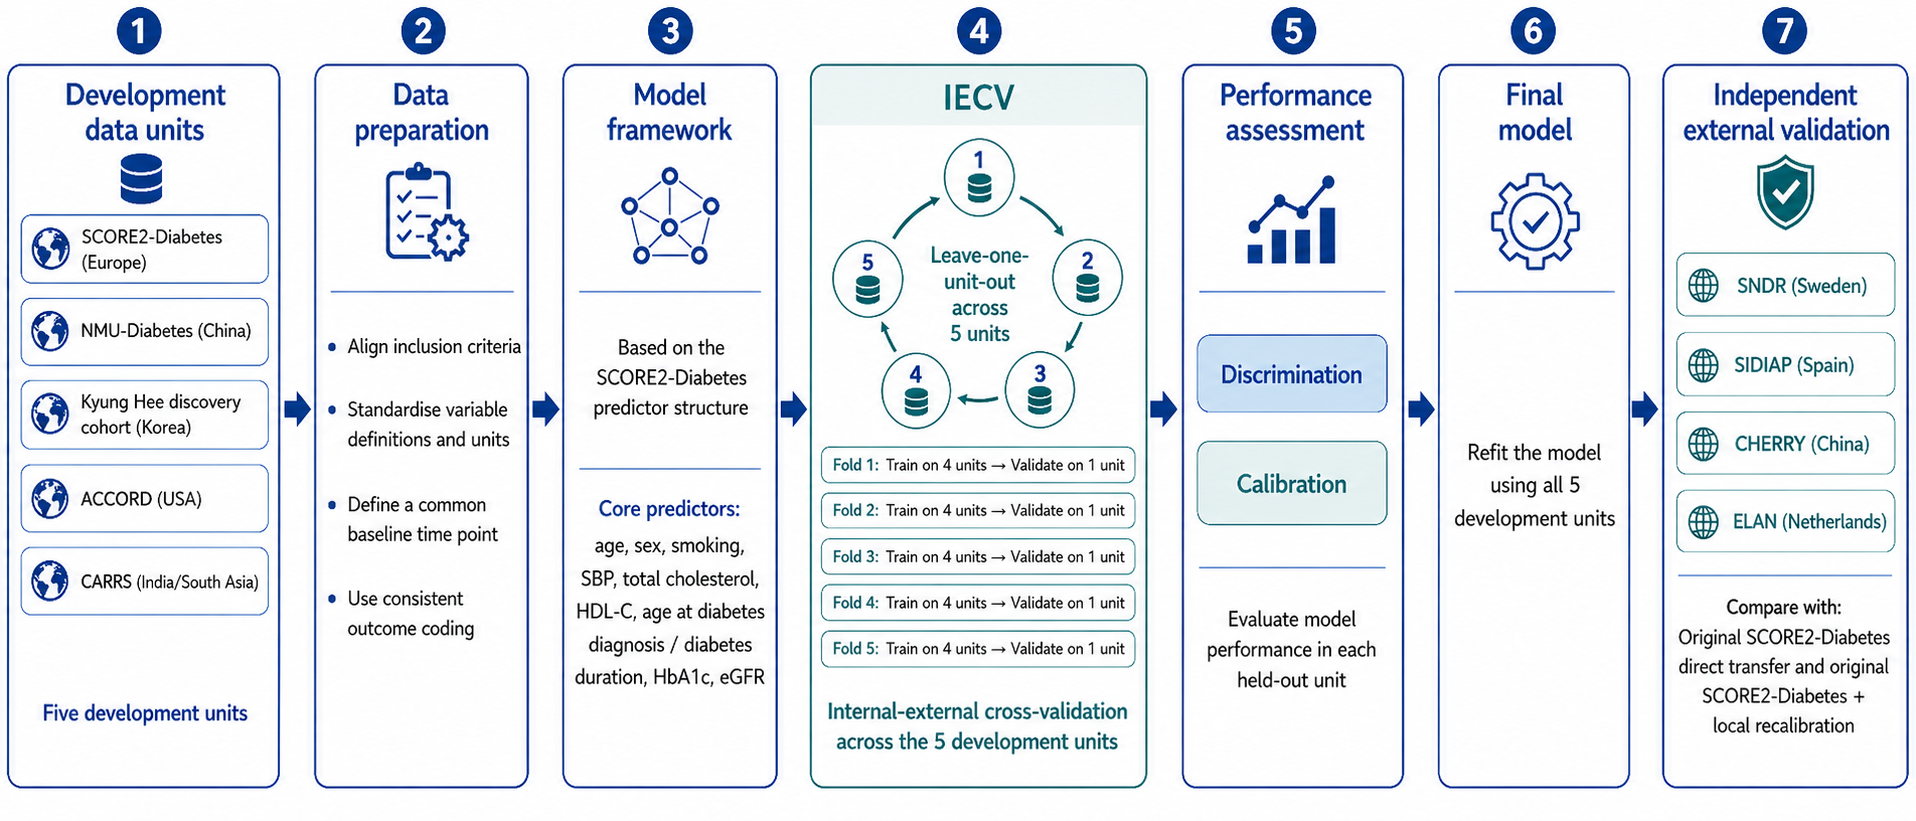
\includegraphics[width=0.7\textwidth]{pipeline.png}
    \caption{Technical pipeline of the proposed multi-region refitting and validation strategy. The framework starts with five development data units, followed by harmonised data preparation, model refitting based on the SCORE2-Diabetes predictor structure, internal-external cross-validation, performance assessment, final model refitting, and independent external validation.}
    \label{fig:pipeline}
\end{figure*}


\section{Research Gap and Objectives }
The above analysis shows that the main limitation of the current T2D CVD risk prediction research is not the lack of models, nor the lack of external verification or model update methods. The more fundamental problem is that most existing models are not designed with robust cross-regional generalisation capabilities as a core goal during development. Although recalibration, revision and expansion can improve the performance of the model in the new population, the repeated use of these methods in different scenarios itself shows that the mobility of the model is still limited. In practice, this means that many models still need to rely on additional local data before reliable use, which increases the burden of implementation and reduces their scalability in clinical scenarios.

Based on this gap, the central research question of this portfolio is:

\begin{quote}
How to design and evaluate a cross-regional modelling and verification strategy for T2D CVD risk prediction, so that the model can better generalise to unseen regional populations while reducing dependence on repeated local calibration?
\end{quote}

To address this question, the study will pursue three objectives:

\begin{enumerate}
    \item Define a unified multi-regional data specification for T2D CVD risk prediction before the 4th week. The specific practice is to map at least five candidate queues to the predictive variable structure of SCORE2 Diabetes, covering the inclusion criteria, prediction variable and outcome definition, follow-up time alignment, acquisition route and data readiness.

    \item By Before the 8th week, develop a cross-regional modelling process based on the structure of SCORE2 Diabetes predictive variables. The process includes multi-regional refitting, standardised preprocessing, missing data processing, and leaving IECV for each development area in turn.

    \item By Week 12, complete a comparative validation framework. The framework compares this strategy with two baselines: direct migration of the original SCORE2 Diabetes model and local recalibration. Comparison indicators include distinction, calibration slope, overall calibration, risk ratio of observed events to expected events, and report results by region.
    
\end{enumerate}

These objectives are feasible within a 12-week portfolio project. Overall, the study aims to test whether a validation-centred cross-region modelling strategy can improve the portability and stability of T2D-CVD risk prediction in unseen populations.




\section{Proposed Methodology}

\subsection{Technical Pipeline}
This study proposes a multi-region refitting strategy designed to improve the transportability of T2D-CVD risk prediction models. The framework starts from the prediction task and core variable structure of SCORE2-Diabetes \cite{score22023score2}, but re-estimates model parameters using harmonised development data from multiple regional sources. The proposed development stage is designed around several candidate data units, including the original SCORE2-Diabetes development datasets and additional T2D cohorts from China, Korea, the United States, and South Asia. These data units are used to expose the model during development to differences in baseline risk, risk factor distributions, clinical measurement practices, and healthcare settings.


As shown in Figure~\ref{fig:pipeline}, before formal modelling, the five development units will be standardised using a common protocol. This process includes four main steps. First, the inclusion criteria will be harmonised by retaining individuals who are comparable to the original SCORE2-Diabetes target population, including people with T2D, no previous CVD, and a consistent age range. Second, variable definitions and measurement units will be standardised. Lipids, HbA1c, kidney function indicators, and smoking status will be coded in the same way, and eGFR will be calculated using a consistent formula. Third, the baseline time point and start of follow-up will be aligned, so that risk factors in each data unit refer to the same prediction starting point. Fourth, outcome definitions and event recording rules will be harmonised. Fatal CVD, non-fatal myocardial infarction, and non-fatal stroke will be coded according to consistent criteria, with clear rules for censoring and competing events. After this standardisation process, the five data units will form a core analysis dataset that can be jointly used for model development.

After data standardisation, internal-external cross-validation will be performed across the five development units. In each round, one data unit will be left out as the validation set, while the remaining four units will be used to refit the model parameters. Model performance will then be assessed in the left-out unit using discrimination and calibration measures. This process will be repeated until each of the five units has served once as an independent external validation set. For example, in the first round, SCID+CPRD+ERFC/UKB, Kyung Hee, ACCORD, and CARRS will be used for training, while NMU-Diabetes will be used for validation. In the second round, the remaining four units will be used for training and Kyung Hee will be used for validation, and so on. Unlike random cross-validation, IECV separates validation units by data source. It therefore more directly simulates the situation in which the model is applied to an unseen region, making it more suitable for evaluating cross-regional transportability.

After the five IECV rounds are completed, and if the strategy shows acceptable cross-regional stability, all five development units will be used to refit a final model. This final model will then be tested in fully independent external validation datasets. The external validation datasets will primarily follow those used in the original SCORE2-Diabetes study and related later studies, including SNDR from Sweden \cite{gudbjornsdottir2003national}, SIDIAP from Spain \cite{bolibar2012sidiap}, and the CHERRY cohort from China \cite{lin2018using}. ELAN from the Netherlands will also be added as an additional validation setting \cite{alfaraj2025external}. These datasets are selected because they have already been used in the literature for independent external validation of SCORE2-Diabetes. Therefore, they can provide a direct point of comparison between the proposed updated model and the original model.


\begin{table*}[t]
\caption{CANDIDATE DATASETS, INTENDED ANALYTICAL ROLE, CORE VARIABLE COVERAGE, AND ACCESS ROUTES.}
\label{tab:planned-datasets}
\centering
\begin{tabular}{l|l|l|l}
\textbf{Data Source}     & \textbf{Use} & \textbf{Core Variable Coverage}                                   & \textbf{Access Route}                         \\ \hline
NMU-Diabetes\cite{wan2022prediction}             & Development  & Published paper reports inclusion of age, HbA1c, eGFR, BP, lipids & Collaborative application                     \\
Kyung Hee cohort (Korea) \cite{sang2024prediction} & Development  & Used in ML prediction study, includes routine clinical variables  & Collaborative access                          \\
ACCORD (USA) \cite{action2008effects}             & Development  & Public data dictionary confirms inclusion of core variables       & Formal application via BioLINCC               \\
CARRS (India) \cite{kondal2022cohort}            & Development  & Literature reports CVD risk factors and T2D variables             & Requires collaboration establishment          \\
SNDR (Sweden) \cite{gudbjornsdottir2003national}            & Validation   & National diabetes registry, covers CVD events and core variables  & Formal application                            \\
SIDIAP (Spain) \cite{bolibar2012sidiap}          & Validation   & Primary care EHR, reported T2D registry variables and outcomes    & Study protocol and ethics approval            \\
CHERRY (China) \cite{lin2018using}          & Validation   & Reported inclusion of SCORE2-Diabetes variable set                & Regional approval \\
ELAN (Netherlands) \cite{alfaraj2025external}       & Validation   & Primary care cohort, used in external validation study            & Protocol and secure environment access       
\end{tabular}
\end{table*}

\subsection{Justification}
The chosen method directly addresses the research objective. The main problem in current T2D-CVD risk prediction is not the lack of models, but the fact that existing models often show performance drift when transferred across regions, especially calibration drift. Therefore, they often require repeated local recalibration to regain usability. SCORE2-Diabetes was selected for two reasons. First, it was developed specifically for people with T2D and includes diabetes-related predictors in addition to conventional cardiovascular risk factors, making it better aligned with the target population of this study. Second, it was developed from multi-country data and has already been externally tested across different regional settings, providing a stronger basis for cross-regional updating than models originally developed for the general population. On this basis, the present study further adopts multi-region refitting and IECV to address regional heterogeneity during the development stage, rather than repeatedly correcting the model only after transport failure. Compared with the usual approach of direct transfer followed by local recalibration, this strategy brings regional heterogeneity into the development stage rather than dealing with it only after model transfer. By refitting the model on multi-region data and testing it in unseen regions using IECV, the study aims to reduce reliance on repeated local recalibration while maintaining acceptable discrimination and calibration across regions.



\subsection{Metrics}
This study will use two types of baseline methods. The first baseline is the direct transfer of the original SCORE2-Diabetes model to the target region. The second baseline is the original SCORE2-Diabetes model after local recalibration in the target region. These two baselines are selected because they represent the two most common pathways for cross-regional model application in the existing literature: direct extrapolation and performance correction through local recalibration after extrapolation. Since the central problem addressed in this study is the dependence of existing models on repeated local recalibration, these two baselines provide the most direct basis for comparison with the proposed method.

Model evaluation will focus on two main aspects: discrimination and calibration. Discrimination will be assessed using Harrell’s C-statistic or AUC, which measures how well the model separates individuals with higher risk from those with lower risk. Calibration will be assessed using calibration plots, the calibration slope, and the agreement between predicted and observed risk. Together, these metrics show whether the model can both rank individuals correctly and produce reliable risk estimates. These measures are widely used in SCORE2-Diabetes and related external validation studies. They are also directly relevant to this study because they capture the main problem of model performance changing across regions. If the proposed multi-region refitting method shows more stable discrimination and calibration across regions than direct transfer, and narrows the performance gap relative to locally recalibrated baselines, it would suggest a more robust approach to cross-regional risk prediction.



\begin{figure*}[htbp]
    \centering
    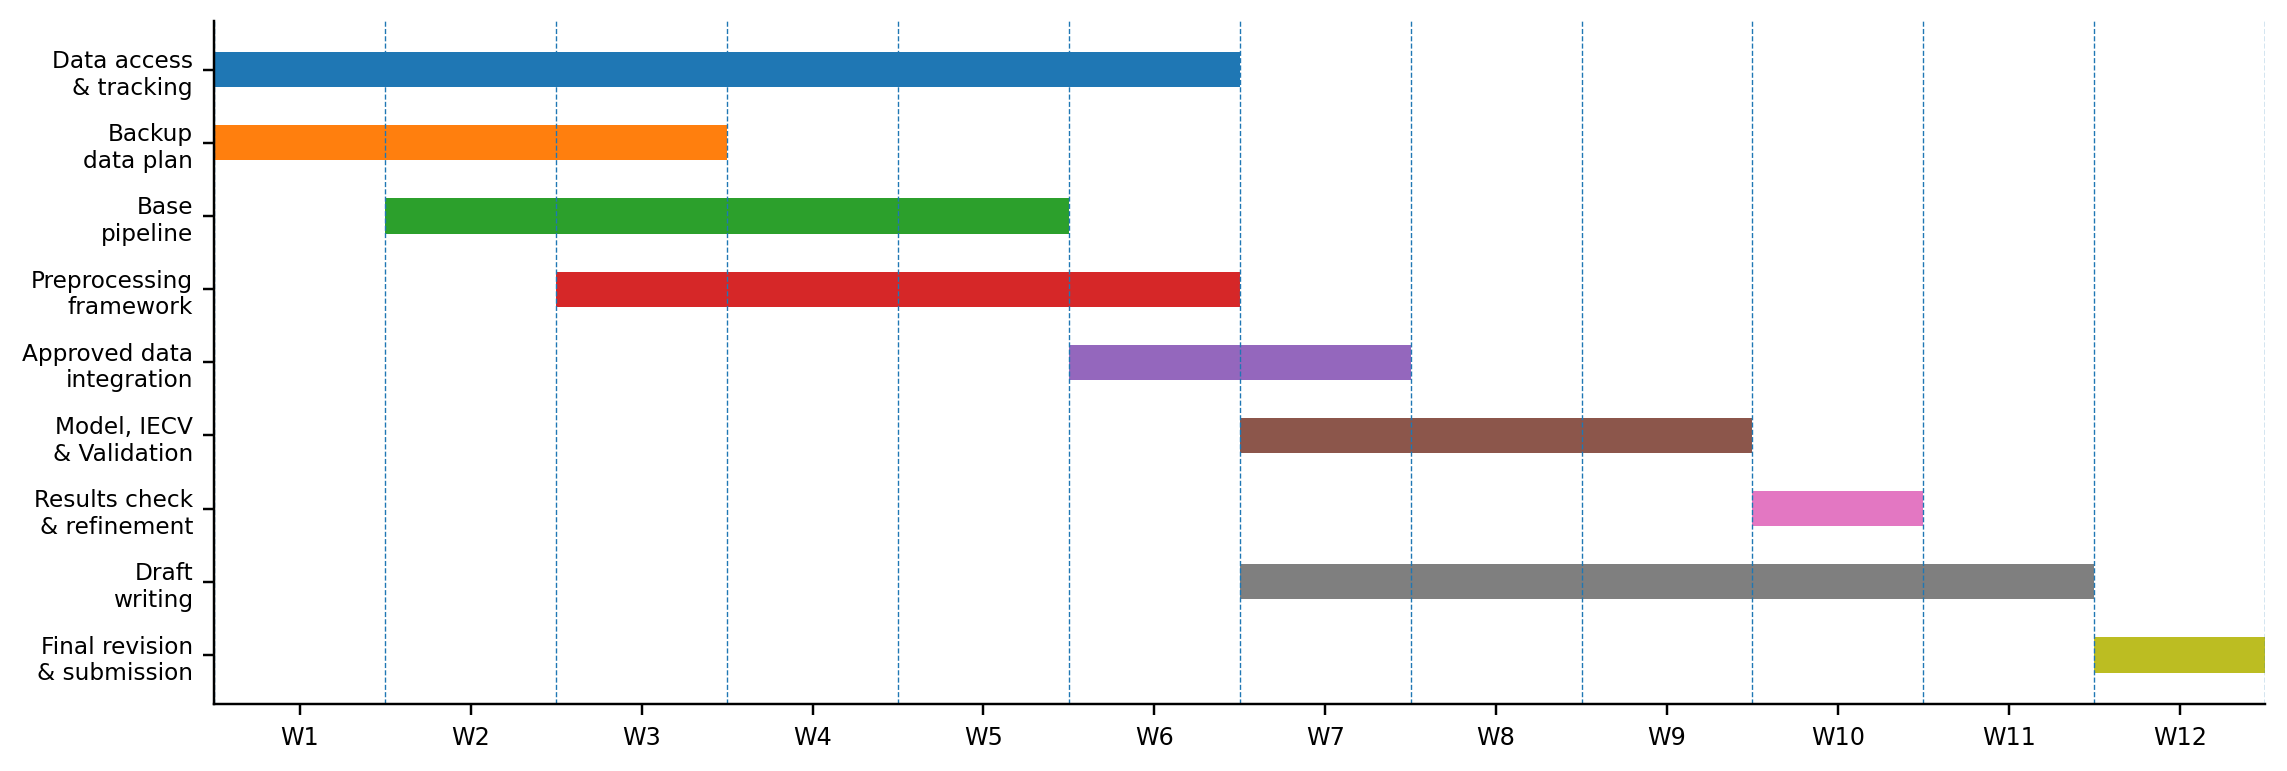
\includegraphics[width=0.65\linewidth]{gantt.png}
    \caption{Gantt chart illustrating the proposed 12-week workflow of the study}
    \label{fig:gantt}
\end{figure*}



\section{Data, Ethics, and Practical Considerations}
\subsection{Data Readiness}
The datasets selected in this study follows four principles. First, the development data set must cover different geographical areas so that the model can be exposed to diversified baseline risks and clinical environments during the training stage. Second, all data sources must provide the set of core variables defined in Section 4. Third, give priority to data sets that have been used in T2D-CVD model development or external verification, which can reduce the uncertainty of variable useability. Fourth, all data sets must be obtained through established applications or cooperation channels.
As shown in Table~\ref{tab:planned-datasets}, this project plans to combine the development and verification data sets of multiple regions. All analyses will be carried out in a formal data use agreement, ethical approval or controlled secure access environment.


\subsection{Ethical Red-Teaming}

This study faces two main risks. The first risk is the imbalance of regional samples. If the European and North American data sets account for too large in the development sample, the model may systematically underestimate or overestimate the risk in the Asian population, even if its overall performance seems acceptable. Previous external verification studies have shown that there are differences in the calibration performance of SCORE2-Diabetes between subgroups with different socio-economic and immigrant backgrounds. Therefore, this problem is not just a theoretical concern. It has been supported by empirical evidence.
The second risk is data heterogeneity. If the variable definitions, measurement methods and result recording rules between different data sets are not fully aligned, the model may learn the differences between different recording systems, not the real cross-regional risk differences. For example, T2D diagnostic time, HbA1c unit, eGFR calculation formula, previous CVD exclusion rules or inconsistency in CVD event coding will directly affect the interpretability of parameter re-fitting and external verification results.



\subsection{Technical Mitigations}
In response to these risks, this study will adopt mitigation strategies from the three levels of data, assessment and governance. At the data level, the main analysis only focusses on those sets of core variables that can be obtained in all data sets and have clear clinical meaning. Inclusion and exclusion criteria, variable definitions, measurement units, baseline time points and result coding will be aligned uniformly to ensure that the model refitting is based on comparable data.
In the evaluation stage, this study will use IECV and independent external verification at the same time. IECV is used to evaluate whether the model can maintain a reasonable distinction and calibration when a certain area is reserved for training data each rotation. Independent external verification will further test the model performance in another data set, and use it to compare the strategy of this study with two common schemes: one is to directly migrate the original SCORE2-Diabetes model, and the other is to recalibrate locally. The performance of each external verification data set will be reported separately, so that any systematic calibration deviations in a specific region or population can be checked, rather than being hidden in the overall average.
At the governance level, all analysis will only be carried out in accordance with the requirements of the relevant data use agreement, ethical approval and secure data environment. This study will also follow the standard principles of data minimisation, purpose limitation and accountability.





\section{Project plan}
Figure~\ref{fig:gantt} shows the 12-week project plan. The project is organised into a phased workflow, corresponding to the above three goals. Weeks 1 to 4 mainly do data access tracking, queue mapping and unified data specification construction. Weeks 4 to 8 mainly do preprocessing design, model re-fitting logic and IECV process. Weeks 8 to 12 mainly do verification design, baseline comparison, performance report, result check and final writing. Since several clinical data sets need to go through the formal application or cooperation agreement process, data access will be started from the first week and treated as a parallel dependency throughout the project. Data sets that have access rights during the project cycle will be included in the modelling and verification process; for data sets that have not been licensed, the corresponding part will be recorded as part of the verification readiness framework.

The project plan is managed using Trello. The board is accessible through the following private link-based access: \url{https://trello.com/invite/b/69f7a98d7f8ea743b8e701da/ATTIfba35f2fa8fa71975dada24742903ec4489CA75A/t2d-cvd-cross-region-modelling-project}






\section{Non-Technical Summary}
Cardiovascular disease is the leading cause of death worldwide. Patients with type 2 diabetes (T2D) have a much higher risk of heart disease and stroke than the general population. For this reason, doctors are increasingly using risk prediction tools to determine which patients may need earlier or more intensive preventive measures. However, tools that perform well in one country or medical system are not necessarily equally useful in another place. Recent guidelines on predictive models point out that when the model is applied to new populations, the performance tends to decline. And the recent external verification of SCORE2-Diabetes in China found that the original model underestimated the cardiovascular risk before recalibration.

This project is aimed at this practical problem. We do not assume that a ready-made model can be migrated directly from one region to another, but propose a strategy: learn from the data of multiple regions at the model development stage, and then check whether the model is still reliable when applied to a new environment. Its goal is not to make a more complex tool, but to make a more reliable tool.

The value of this work is mainly reflected in the practical level. If cardiovascular risk can be more consistently estimated among different populations, clinicians can make more accurate decisions about prevention, follow-up and treatment intensity. This is especially important in type 2 diabetes, because missing or underestimating the risk can lead to delaying the action of patients who should have benefitted from early intervention. A more robust cross-regional approach can also reduce the need to repeatedly adjust the model every time a new population is introduced, making the implementation of the medical system and researchers more efficient.

Overall, the proposed work seeks to improve the fairness, reliability, and real-world usefulness of cardiovascular risk prediction for people with T2D across different regions.




\bibliographystyle{IEEEtran}
\bibliography{references}

\end{document}
